%%%% Dokumentklassen %%%%

\documentclass[a4paper,11pt,fleqn,dvipsnames,twoside,openany]{memoir} 	% Openright åbner kapitler på højresider (openany begge)


%%%% PACKAGES %%%%

%% Oversættelse og tegnsætning %%
\usepackage[utf8]{inputenc}					% Input-indkodning af tegnsæt (UTF8)
\usepackage[danish]{babel}					% Dokumentets sprog
\usepackage[T1]{fontenc}					    % Output-indkodning af tegnsæt (T1)
\usepackage{ragged2e,anyfontsize}			% Justering af elementer
\usepackage{fixltx2e}						% Retter forskellige fejl i LaTeX-kernen

\usepackage{lastpage}						% Total antal sider opdateres automatisk ved \pageref{LastPage}
																			
%% Figurer og tabeller (floats) %%
\usepackage{graphicx} 						% Håndtering af eksterne billeder (JPG, PNG, EPS, PDF)
\usepackage{multicol}         	            	% Muliggør output i spalter
\usepackage{rotating}						% Rotation af tekst med \begin{sideways}...\end{sideways}
\usepackage{xcolor}							% Definer farver med \definecolor. Se mere: http://en.wikibooks.org/wiki/LaTeX/Colors
\usepackage{flafter}						% Sørger for at floats ikke optræder i teksten før deres reference
\let\newfloat\relax 						% Justering mellem float-pakken og memoir
\usepackage{float}							% Muliggør eksakt placering af floats, f.eks. \begin{figure}[H]

%% Matematik mm. %%
\usepackage{amsmath,amssymb,stmaryrd} 		% Avancerede matematik-udvidelser
\usepackage{mathtools}						% Andre matematik- og tegnudvidelser
\usepackage{textcomp}                 		% Symbol-udvidelser (fx promille-tegn med \textperthousand)
\usepackage{rsphrase}						% Kemi-pakke til RS-saetninger, fx \rsphrase{R1}
\usepackage[version=3]{mhchem} 				% Kemi-pakke til flot og let notation af formler, f.eks. \ce{Fe2O3}
\usepackage{siunitx}						% Flot og konsistent præsentation af tal og enheder med \si{enhed} og \SI{tal}{enhed}
\sisetup{output-decimal-marker = {,}}		% Opsætning af \SI (DE for komma som decimalseparator) 

%% Referencer og kilder %%
\usepackage[danish]{varioref}				% Muliggør bl.a. krydshenvisninger med sidetal (\vref)
\usepackage{natbib}							% Udvidelse med naturvidenskabelige citationsmodeller
\usepackage{xr}							    % Referencer til eksternt dokument med \externaldocument{<NAVN>}

%% Misc. %%
\usepackage{listings}						% Placer kildekode i dokumentet med \begin{lstlisting}...\end{lstlisting}
\usepackage{lipsum}							% Dummy text \lipsum[..]
\usepackage[shortlabels]{enumitem}			% Muliggør enkelt konfiguration af lister
\usepackage{pdfpages}						% Gør det muligt at inkludere pdf-dokumenter med kommandoen \includepdf[pages={x-y}]{fil.pdf}	
\pdfoptionpdfminorversion=6					% Muliggør inkludering af pdf-dokumenter, af version 1.6 og højere
\pretolerance=2500 							% Justering af afstand mellem ord (højt tal, mindre orddeling og mere luft mellem ord)


%%%% CUSTOM SETTINGS %%%%

%% Marginer %%
\setlrmarginsandblock{3.5cm}{2.5cm}{*}		% \setlrmarginsandblock{Indbinding}{Kant}{Ratio}
\setulmarginsandblock{2.5cm}{3.0cm}{*}		% \setulmarginsandblock{Top}{Bund}{Ratio}
\checkandfixthelayout 						% Oversætter værdier til brug for andre pakker

%% Afsnitsformatering %%
\setlength{\parindent}{0mm}           		% Størrelse af indryk
\setlength{\parskip}{3mm}          			% Afstand mellem afsnit ved brug af double Enter
\linespread{1,1}							% Linjeafstand

%% Indholdsfortegnelse %%
\setsecnumdepth{subsection}		 			% Dybden af nummererede overskrifter (part/chapter/section/subsection)
\maxsecnumdepth{subsection}					% Dokumentklassens grænse for nummereringsdybde
\settocdepth{subsection} 					% Dybden af indholdsfortegnelsen
		
%% Opsætning af listings %%
\definecolor{commentGreen}{RGB}{34,139,24}
\definecolor{stringPurple}{RGB}{208,76,239}

\lstset{language=Matlab,					    % Sprog
	basicstyle=\ttfamily\scriptsize,		    % Opsætning af teksten
	keywords={for,if,while,else,elseif,		% Nøgleord at fremhæve
			  end,break,return,case,
			  switch,function},
	keywordstyle=\color{blue},				% Opsætning af nøgleord
	commentstyle=\color{commentGreen},		% Opsætning af kommentarer
	stringstyle=\color{stringPurple},		% Opsætning af strenge
	showstringspaces=false,					% Mellemrum i strenge enten vist eller blanke
	numbers=left, numberstyle=\tiny,		    % Linjenumre
	extendedchars=true, 					    % Tillader specielle karakterer
	columns=flexible,						% Kolonnejustering
	breaklines, breakatwhitespace=true,		% Bryd lange linjer
}

%% Navngivning %%
\addto\captionsdanish{
	\renewcommand\appendixname{Appendiks}
	\renewcommand\contentsname{Indholdsfortegnelse}	
	\renewcommand\appendixpagename{Appendiks}
	\renewcommand\appendixtocname{Appendiks}
	\renewcommand\cftchaptername{\chaptername~}		% Skriver "Kapitel" foran kapitlerne i indholdsfortegnelsen
	\renewcommand\cftappendixname{\appendixname~}	% Skriver "Appendiks" foran appendiks i indholdsfortegnelsen
}

%% Kapiteludssende %%
\definecolor{numbercolor}{gray}{0.7}		            % Definerer en farve til brug til kapiteludseende
\newif\ifchapternonum

\makechapterstyle{jenor}{					        % Definerer kapiteludseende frem til ...
  \renewcommand\beforechapskip{0pt}
  \renewcommand\printchaptername{}
  \renewcommand\printchapternum{}
  \renewcommand\printchapternonum{\chapternonumtrue}
  \renewcommand\chaptitlefont{\fontfamily{pbk}\fontseries{db}\fontshape{n}\fontsize{25}{35}\selectfont\raggedleft}
  \renewcommand\chapnumfont{\fontfamily{pbk}\fontseries{m}\fontshape{n}\fontsize{1in}{0in}\selectfont\color{numbercolor}}
  \renewcommand\printchaptertitle[1]{%
    \noindent
    \ifchapternonum
    \begin{tabularx}{\textwidth}{X}
    {\let\\\newline\chaptitlefont ##1\par} 
    \end{tabularx}
    \par\vskip-2.5mm\hrule
    \else
    \begin{tabularx}{\textwidth}{Xl}
    {\parbox[b]{\linewidth}{\chaptitlefont ##1}} & \raisebox{-15pt}{\chapnumfont \thechapter}
    \end{tabularx}
    \par\vskip2mm\hrule
    \fi
  }
}											        % ... her

\chapterstyle{jenor}						        % Valg af kapiteludseende - Google 'memoir chapter styles' for alternativer

%% Sidehoved %%

\makepagestyle{AAU}							        % Definerer sidehoved og sidefod udseende frem til ...
\makepsmarks{AAU}{%
	\createmark{chapter}{left}{shownumber}{}{. \ }
	\createmark{section}{right}{shownumber}{}{. \ }
	\createplainmark{toc}{both}{\contentsname}
	\createplainmark{lof}{both}{\listfigurename}
	\createplainmark{lot}{both}{\listtablename}
	\createplainmark{bib}{both}{\bibname}
	\createplainmark{index}{both}{\indexname}
	\createplainmark{glossary}{both}{\glossaryname}
}
\nouppercaseheads									% Ingen Caps ønskes

\makeevenhead{AAU}{\small ST3PRJ3 Gruppe 2}{}{\leftmark}	% Definerer lige siders sidehoved (\makeevenhead{Navn}{Venstre}{Center}{Hoejre})
\makeoddhead{AAU}{\rightmark}{}{\small ASE}		            % Definerer ulige siders sidehoved (\makeoddhead{Navn}{Venstre}{Center}{Højre})
\makeevenfoot{AAU}{\small \thepage}{}{}						% Definerer lige siders sidefod (\makeevenfoot{Navn}{Venstre}{Center}{Højre})
\makeoddfoot{AAU}{}{}{\small \thepage}						% Definerer ulige siders sidefod (\makeoddfoot{Navn}{Venstre}{Center}{Højre})

\copypagestyle{AAUchap}{AAU}							% Sidehoved for kapitelsider defineres som standardsider, men med blank sidehoved
\makeoddhead{AAUchap}{}{}{}
\makeevenhead{AAUchap}{}{}{}
\makeheadrule{AAUchap}{\textwidth}{0pt}
\aliaspagestyle{chapter}{AAUchap}					% Den ny style vælges til at gælde for chapters
													% ... her
															
\pagestyle{AAU}										% Valg af sidehoved og sidefod


%%%% CUSTOM COMMANDS %%%%

%% Billede hack %%
\newcommand{\figur}[4]{
		\begin{figure}[H] \centering
			\includegraphics[width=#1\textwidth]{billeder/#2}
			\caption{#3}\label{#4}
		\end{figure} 
}

%% Specielle tegn %%
\newcommand{\decC}{^{\circ}\text{C}}
\newcommand{\dec}{^{\circ}}
\newcommand{\m}{\cdot}


%%%% ORDDELING %%%%

\hyphenation{}


%%%% Tilføjelser af min preample %%%%

% Booktabs:
% The booktabs package is needed for better looking tables. 
\usepackage{booktabs}

% Caption:
% For better looking captions. See caption documentation on how to change the format of the captions.
\usepackage[hang, font={small, it}]{caption}

% Hyperref:
% This package makes all references within your document clickable. By default, these references will become boxed and colored. This is turned back to normal with the \hypersetup command below.
\usepackage{hyperref}
	\hypersetup{colorlinks=false,pdfborder=0 0 0}

% Cleveref:
% This package automatically detects the type of reference (equation, table, etc.) when the \cref{} command is used. It then adds a word in front of the reference, i.e. Fig. in front of a reference to a figure. With the \crefname{}{}{} command, these words may be changed.
\usepackage{cleveref}
	\crefname{equation}{formel}{formler}
	\crefname{figure}{figur}{figurer}	
	\crefname{table}{tabel}{tabeller}

% Mine tilføjelser:
\usepackage{units}                        %% Bruges til at gøre fx 1/2 samlet med: \nicefrac{1}{2}.
\usepackage{tabu, longtable}              %% Bruges til tabeller.
\setlength{\tabulinesep}{1.5ex}           %% Definerer linjeafstand i tabeller.
\usepackage{enumerate}                    %% Bruges til lister.
\usepackage{tabto}                        %% Giver mulighed for TAB med fx \tabto{3em}.
\usepackage[hyphenbreaks]{breakurl}       %% Bruges til websiders url'er.
\renewcommand{\UrlFont}{                  %% Definerer url-font.
\small\ttfamily}                          %
\bibliographystyle{unsrt}                 %% Definere bibliografien. Ses til sidst i dokumentet i kapitlet Litteratur.
\usepackage{amssymb} 
\usepackage{pifont}
%\newcommand{\xmark{\ding{55}}			 % Opretter et unchecked mark
\raggedbottom

%\externaldocument[D-]{Dokumentation}

\begin{document}	
\frontmatter						% Nummereres med romerske tal.
\begin{titlingpage}
\begin{center}

~ \\[3cm]


\includegraphics[width=0.6\textwidth]{figurer/ASE}~\\[1cm]

\textsc{\LARGE Aarhus School of Engineering}\\[1.5cm]

\textsc{\Large Sundhedsteknologi}\\
\textsc{\Large 3. semesterprojekt}\\[0.5cm]

\noindent\makebox[\linewidth]{\rule{\textwidth}{0.4pt}}\\
[0.5cm]{\Huge Rapport}
\noindent\makebox[\linewidth]{\rule{\textwidth}{0.4pt}}

\end{center}



\textit{Gruppe 2} \newline
Anne Bundgaard Hoelgaard\tab(201404492) \newline
Mette Hammer Nielsen-Kudsk\tab(201408391) \newline
Ditte Heebøll Callesen\tab(201408392) \newline	
Martin Banasik\tab(201408398) \newline	
Albert Jakob Fredshavn\tab(201408425) \newline 
Johan Mathias Munk\tab(201408450) \newline 




\textit{Vejleder:} \newline
Studentervejleder\\
Peter Johansen\\
Aarhus Universitet


\vfill

\begin{center}
{\large 16. december 2015}
\end{center}


\end{titlingpage}
%\include{Rfiler/Resume}
\begin{vplace}[0.6]
{\large \textit{Gruppemedlemmer}}
\\
\\

\noindent \begin{tabular}{ll}
	\makebox[3.0in]{\hrulefill} & \makebox[1.5in]{\hrulefill}\\
	Albert Jakob Fredshavn  (201408425) & Dato\\[7ex]% adds space between the two sets of signatures
	\makebox[3in]{\hrulefill} & \makebox[1.5in]{\hrulefill}\\
	Ditte Heebøll Callesen  (201408392) & Dato\\[7ex]
	\makebox[3in]{\hrulefill} & \makebox[1.5in]{\hrulefill}\\
	Martin Banasik  (201408398) & Dato\\[7ex]
	\makebox[3in]{\hrulefill} & \makebox[1.5in]{\hrulefill}\\
	Mette Hammer Nielsen-Kudsk  (201408391) & Dato\\[7ex]
	\makebox[3in]{\hrulefill} & \makebox[1.5in]{\hrulefill}\\
	Johan Mathias Munk  (201408450) & Dato\\[7ex]
	\makebox[3in]{\hrulefill} & \makebox[1.5in]{\hrulefill}\\
	Anne Bundgaard Hoelgaard (201404492) & Dato\\[7ex]
	
	
\end{tabular}
\\
{\large \textit{Vejleder}}
\\
\\
\\
\noindent \begin{tabular}{ll}
	\makebox[3.0in]{\hrulefill} & \makebox[1.5in]{\hrulefill}\\
	Peter Johansen & Dato\\[8ex]
\end{tabular}
\end{vplace}

\chapter{Godkendelsesformular}

{\LARGE\textit{Godkendelsesformular}}

{\large Forfattere:}
\\[5ex]


\begin{tabular}{c c}
\centering 
	\makebox[2.0in]{\hrulefill} & \makebox[2.0in]{\hrulefill}\\
	Albert Jakob Fredshavn & Ditte Heebøll Callesen\\[7ex]
	\makebox[2.0in]{\hrulefill} & \makebox[2.0in]{\hrulefill}\\
	Martin Banasik & Mette Hammer Nielsen-Kudsk\\[7ex]
	\makebox[2.0in]{\hrulefill} & \makebox[2.0in]{\hrulefill}\\
	Johan Mathias Munk & Anne Bundgaard Hoelgaard\\[7ex]
	

\end{tabular}

\begin{tabular}{c c c c}
	\textbf{Godkendes af} & Peter Johansen\\[3ex]
	\textbf{Antal sider} & c \\[3ex]
	\textbf{Kunde} & Aarhus Universitet
\end{tabular}\\[8ex]
Ved underskrivelse af dette dokument accepteres det af begge parter som værende kravene til udviklingen af det ønskede system.
\\
\\
\textbf{Dato: } 16/12-2015\\[7ex]

\begin{tabular}{c c}
	\makebox[2.0in]{\hrulefill} & \makebox[2.0in]{\hrulefill}\\
	\centering 
	Kundens underskrift & Leverandørens underskrift
\end{tabular}

%\chapter{Ordliste}

\begin{longtabu} to \linewidth{@{}l X[j]@{}}
    Ord &    Forklaring\\
    \toprule\
(F)URPS+ 	&    Et akronym, der repræsenterer en model til klassificering af softwarens kvalitet \\
    GUI		&	Graphical User Interface (Grafisk brugergrænseflade)\\
    VPN		&	Virtual Private Network\\
    DAQ		&	Data acquisition \\
    SysML	&   Systems Modeling Language – sprog til visuel fremstilling af systemer \\
    UML		& Unified modelling language – sprog til oversigtsfremstilling af klasser i programmering \\
    KSS		&	Kommunikation og Samarbejde i Sundhedsvæsnet \\
    BDD 	&	Block Defination Diagram \\
	IBD		& 	Intern Block Diagram \\
	SD		& 	Sekvensdiagram \\
	UML		& 	Unified Modeling Language \\
	ISE 	&	Indledende System Engineering \\
	Hjerteinsufficiens &  Hjertesvigt \\
	DSB		&	Digital Signalbehandling \\
	Hypertension &  Forhøjet blodtryk \\
	Hypotension & Lavt blodtryk \\
	MTTR	&	Mean Time To Restore \\
	MTBF	&	Mean Time Between Failure \\
 
\label{forkort}
\end{longtabu}
\cleardoublepage		

\tableofcontents*                   % Indsætter en indholdsfortegnelse før Indledning.

\mainmatter                         % Her findes de nummererede kapitler modsat \frontmatter og \backmatter. Nummereres med arabiske tal.
%
\chapter{Indledning}
I dette projekt arbejdes der med blodtryksmålere. Vi har valgt at udarbejde en blodtryksmåler til forskningsbrug. Blodtryksmåleren skal kunne modtage en spænding fra en transducer, nulpunktsjustere og kalibere efter en forskers ønske. Signalet skal vises i en graf, på et display, hvor værdier for puls, systoliske- og diastoliske tryk vises. Her fra forskeren starter og gemmer sine målinger.\\
I kravspecifikationen findes de krav, der er blevet stillet for projektet. Herunder er også de krav, som blev stillet mellem os og vores vejleder.\\
Under systemarkitekturen findes informationer om, hvordan software- og hardwaredelen er opbygget.  I afsnittet integrationstest kan der læses om, hvordan projektet er blevet testet.\\  

\subsubsection{Versionshistorik}

\begin{longtabu} to \linewidth{@{}l l l X[j]@{}}
    Version &    Dato &    Ansvarlig &    Beskrivelse\\[-1ex]
    \midrule
    0.1 &   04-11-2015	&   MHNK  &   Oprettelse af LaTex dokumenter \\
    0.2 &   11-11-2015	&   ABH  &   Udviklingsværktøjer og krav \\
    0.3 &   11-11-2015	&   DHC  &   Metoder \\
    0.4 &   18-11-2015	&   ABH  &   Systembeskrivelse  \\
    0.5 &   19-11-2015	&   DHC  &   Perspektivering - Fremtidigt arbejde \\
    0.6 &   24-11-2015	&   MHNK  &   Blodtryk \\
    0.7 &   24-11-2015	&   AJF  &   Projektgennemførelse og -styring \\
    0.8 &   24-11-2015	&   MM  &   Projektformulering og afgrænsning \\
    1.0 &   01-12-2015	&   MB, MHNK  &   Referencelister i LaTex \\
    1.1 &   02-12-2015	&   MB, MHNK  &   Figurlister i LaTex \\
    1.2 &   02-12-2015	&   MHNK  &   Resume \\
    1.3 &   07-12-2015	&   MHNK  &   Abstract \\
    1.4 &   09-12-2015	&   MHNK  &   Konklusion \\
   
    	
\label{version_Systemark}
\end{longtabu}
%\chapter{Problemformulering og afgrænsning}
\subsubsection{Ansvarsområder}

Idet gruppens størrelse ikke lægger op til samlet, at arbejde på alle dele på samme tid, er projektets ansvarsområder blevet fordelt som følgende:

\begin{longtabu} to \linewidth{@{}l l l X[j]@{}}
    Navn &    Ansvarsområder &    \\[-1ex]
    \midrule
    Ditte Heebøll Callesen &   Hardwaredesign, dokumentation	&    \\
    Albert Jakob Fredshavn &   Hardwaredesign, dokumentation	&    \\
    Martin Banasik         &   Hardwaredesign, dokumentation	&    \\
    Johan Mathias Munk     &   Softwaredesign, algoritmeopbygning, dokumentation &    \\
    Mette Hammer Nielsen-Kudsk  &   Softwaredesign, algoritmeopbygning, dokumentation	&    \\
   	Anne Hoelgaard    &   Softwaredesign, algoritmeopbygning, dokumentation	&    \\
\label{version_Systemark}
\end{longtabu}
%\include{Rfiler/Rbaggrund}
%\chapter{Systembeskrivelse}
Med udgangspunkt i projektformuleringen kommer dette projekts endelige system til at bestå af et software og hardware system, der kan tilsluttes et måleobjekt, hvorpå et blodtryk kan måles. Systemet skal kunne implementeres i forskningsmiljøer, hvor en eller flere forskere ønsker at analysere indhentede blodtrykssignaler. Visionen er, at systemet skal være let tilgængeligt og effektivt, hvilket vil komme til udtryk ved, at systemet fungerer stabilt.

I dette projekt realiseres en prototype af systemet. Det vil sige at flere dele af systemet udvikles ud fra forsimplede metoder ift. hvordan det vil være optimalt at implementere dem i virkeligheden. Her tænkes på hardware-, såvel som software-elementer. Hardwaren i prototypen realiseres på et VEVO Board, så det er muligt at tage den med sig, samt er mere holdbar over tid. Softwaren i prototypen består af flere moduler. Disse er opbygget efter principperne i en trelagsmodel, hvilket vil sige, at koden indeholder et database-lag, logik-lag samt præsentations-lag. Dette er valgt for, at skabe et overblik over hvilke dele af software-koden der har ansvaret for de enkelte funktionaliteter i systemet.

Hardwaren består af en forstærker og et filter. Forstærkerens opgave består i at forstærke det analoge signal fra max 11 millivolt til 5 volt. Filtret sørger for at filtrere unødigt støj fra det analog signal. Signalændringen fra måleobjektet til visning af signal på en graf er skitseret herunder. Det skal pointeres at dette kun er en skitse for at skabe overblik, derfor er flere processer i softwaren udeladt af diagrammet. 
\begin{figure}[htb]
	\centering
	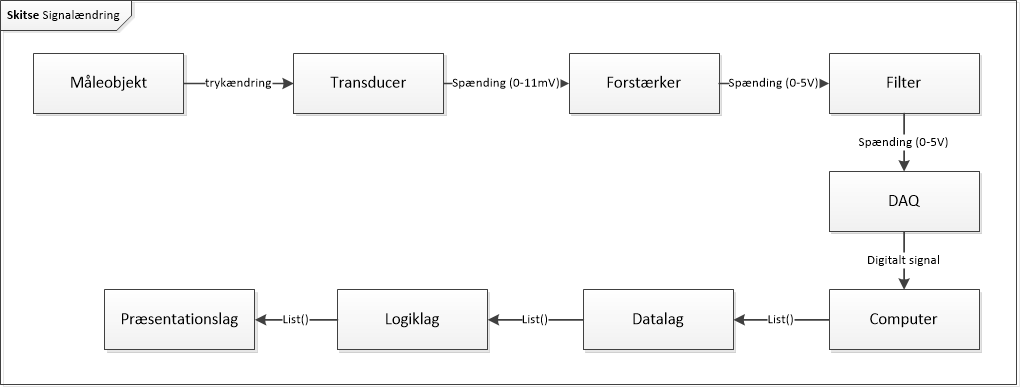
\includegraphics[width=1.0\textwidth]{Figurer/Signalandring}
	\caption{Skitse af signalændring}
	%\label{fig:Skitse der viser signalændring}
\end{figure}
Database-laget består af en lukket database samt indhentningen af blodtrykssignalet fra måleobjektet til transduceren, gennem hardware, inden det rammer software-delen. I den lukkede database gemmes det indhentede blodtrykssignal i en tabel. Signalet gemmes med et tidsstempel, samt under et autogenereret Id, sammensat med det forsøgsnavn som forskeren indtaster på brugergrænsefladen ved begyndelsen af en måling. \\
Logik-laget er handlingslaget, og alt kommunikation til de resterende lag går gennem dette lag. Laget indeholder flere klasser, der indeholder metoder til indhentning af systoliske-, diastoliske og puls-værdier, ud fra det indhentede blodtrykssignal. Derudover indeholder laget også klasser, der har ansvaret for at foretage en filtrering af signalet når dette er valgt. \\ 
Præsentationslaget er forskerens vej ind i systemet, dette lag har til ansvar, at udskrive valgte data på brugergrænsefladen. 

Systemet skal udadtil have en brugergrænseflade i form af en touch skærm eller almindelig computerskærm med tilhørende tastatur. Det er denne skærm som den primære aktører til systemet, altså forskeren, interagerer med. Det tilstræbes, at opbygge brugergrænsefladen simpelt og efter forskerens logik, så opbygningen giver mening for systemets bruger. Efter indhentning af blodtrykssignal er systemet i stand til grafisk at vise signalet kontinuerligt, samt udskrive blodtrykssignalets systoliske-, diastoliske- og puls-værdier. 

%\chapter{Krav}

%\chapter{Projektbeskrivelse}
\subsection{Projektgennemførelse}
\subsubsection{Projektstyring}

\subsection{Metoder}
I tråd med ASE-modellen(beskrevet i Projektgennemførelse) er der blevet brugt accepttest, til at teste produktet.  
\subsection{Systemarkitektur}
\subsubsection{Hardware}
\subsubsection{Software}

\subsection{Problemidentifikation (design)}
\subsubsection{Hardware}
\subsubsection{Software}

\subsection{Implementering}
\subsubsection{GUI-beskrivelse}
\subsubsection{Algoritmer (grænseværdier)}
\subsubsection{Filteret/Ufiltreret}
\subsubsection{Lagring af data i Database}

\subsection{Test}
\subsection{Resultater og diskussion}
\subsection{Udviklingsværktøjer}
Gennem projektarbejdet har vi anvendt en række forskellige værktøjer til udvikling af blodtryksmåler-systemet. Disse er yderligere uddybet herunder.

\textbf{Visual Studio 2013}

Softwaredelen af projektets programmering er skrevet i sproget C-sharp. Her er Visual Studio 2013 anvendt som kompiler, da programmet gør det nemt at omskrive tekst til kode. Visual Studio 2013 indeholder også funktionen Windows Form Application, der visuelt kan fremstillede de ønskede resultater i form af knapper, grafer og labels mv. i en samlet brugergrænseflade, som aktøren interagerer med. 

\textbf{Microsoft Visio 2016}

Microsoft Visio er et tegne værktøj, der i dette projekt er anvendt til at designe både SysML og UML diagrammer, som benyttes ved organisering af hardware og software design. Microsoft Visio er det oplagte valg, da diagrammer lavet i programmet får et enkelt og overskueligt udseende, og dermed fremstår det tydeligt for læseren hvad diagrammet vil vise.

\textbf{Analog Discovery og Waveform fra Digilent}

Analog Discovery og waveform er i projektet benyttes som omformer og signal generator under testfasen. Her fungerer Analog Discovery som en waveform generator, så et analog signal kan sendes videre ind i lavpasfiltret, forstærkeren og derefter ind i DAQ’en. I den endelig implementering erstattes Analog Discovery og Waveform med transduceren. 

\textbf{NI-DAQmx}

NI-DAQmx er et værktøj udarbejdet af National Instruments, som anvendes til at omforme det indkomne analoge signal fra transduceren (Analog Discovery) til et digital signal. Værdier fra NI-DAQmx er af en type som kan anvendes i selve softwarekoden. 

\textbf{LaTeX}

LaTeX er anvendt i projektet til design og opsætning af projektrapport og projektdokumentation. LaTeX er god til tekstformatering, hvor opsætning og strukturer defineres samlet for hele en rapport, samt god til versionsstyring. Til at skrive selve koden benyttes programmet TeX-maker som kombiler. 

\subsection{Opnåede resultater}
\subsection{Perspektivering - Fremtidigt arbejde}
I fremtiden vil blodtryksmåleren kunne udviges gennem flere muligheder. Da blodtryksmåleren er lavet til forskningsbrug, er der ingen idé i at udvide mod patienter.  En forlængelse af systemet kunne derimod være en metode, som skal kunne vise gemte målinger. \newline Et log-in vindue er en anden ting som kunne forbedre systemet, for på den måde at skabe større sikkerhed for forskeren og dataen. Et log-in vindue vil gøre at, en forsker kan være sikker på at hans målinger og forskning ikke kan tilgås af andre. Det kræver en større udvidelse, hvor der skal laves et log-in vindue og en database, hvor password og brugernavn gemmes. Der skal også laves en metode, som kan tjekke om det indtastede password og brugernavn passer over ens med det i databasen. 
\newline
Generelt skal de standarter, som findes for blodtryksmålere undersøges grundigere. Specielt brugergrænsefladen, men også resten af systemet som enheder og visning af graf, skal rettes til efter de passende standarter.
\newline 
Fremtidsaspekter kunne også være, hvis systemet kunne tilpasses forskning mere.  Det kunne være gennem bedre navngivning af data eller et bedre overblik over, hvordan data bliver gemt, fx gennem en liste for de gemte målinger.   
%\chapter{Konklusion}

%\chapter{Referencer}


\backmatter


%\bibliography{bibliografi/PRJ3}    % Sætter bibliografien bagerst i dokumentet. Bruger bib-filen PRJ3.

\end{document}